%% LyX 2.2.3 created this file.  For more info, see http://www.lyx.org/.
%% Do not edit unless you really know what you are doing.
\documentclass[12pt,english]{article}
\usepackage[osf]{mathpazo}
\renewcommand{\sfdefault}{lmss}
\renewcommand{\ttdefault}{lmtt}
\usepackage[T1]{fontenc}
\usepackage[latin9]{inputenc}
\usepackage[paperwidth=30cm,paperheight=35cm]{geometry}
\geometry{verbose,tmargin=2cm,bmargin=2cm}
\setlength{\parindent}{0bp}
\usepackage{amsmath}
\usepackage{amssymb}

\makeatletter

%%%%%%%%%%%%%%%%%%%%%%%%%%%%%% LyX specific LaTeX commands.
%% Because html converters don't know tabularnewline
\providecommand{\tabularnewline}{\\}

%%%%%%%%%%%%%%%%%%%%%%%%%%%%%% User specified LaTeX commands.
\usepackage{tikz}
\usetikzlibrary{matrix,arrows,decorations.pathmorphing}
\usetikzlibrary{shapes.geometric}
\usepackage{tikz-cd}
\usepackage{amsthm}
\usepackage{xparse,etoolbox}

\theoremstyle{plain}
\newtheorem{theorem}{Theorem}[section]
\newtheorem{lemma}[theorem]{Lemma}
\newtheorem{prop}{Proposition}[section]
\newtheorem*{cor}{Corollary}
\theoremstyle{definition}
\newtheorem{defn}{Definition}[section]
\newtheorem{ex}{Exercise} 
\newtheorem{example}{Example}[section]
\theoremstyle{remark}
\newtheorem*{rem}{Remark}
\newtheorem*{note}{Note}
\newtheorem{case}{Case}
\usepackage{graphicx}
\usepackage{amssymb}
\usepackage{tikz-cd}
\usetikzlibrary{calc,arrows,decorations.pathreplacing}
\tikzset{mydot/.style={circle,fill,inner sep=1.5pt},
commutative diagrams/.cd,
  arrow style=tikz,
  diagrams={>=latex},
}

\usepackage{babel}
\usepackage{hyperref}
\hypersetup{
    colorlinks,
    citecolor=blue,
    filecolor=blue,
    linkcolor=blue,
    urlcolor=blue
}
\usepackage{pgfplots}
\usetikzlibrary{decorations.markings}
\pgfplotsset{compat=1.9}


\newcommand{\blocktheorem}[1]{%
  \csletcs{old#1}{#1}% Store \begin
  \csletcs{endold#1}{end#1}% Store \end
  \RenewDocumentEnvironment{#1}{o}
    {\par\addvspace{1.5ex}
     \noindent\begin{minipage}{\textwidth}
     \IfNoValueTF{##1}
       {\csuse{old#1}}
       {\csuse{old#1}[##1]}}
    {\csuse{endold#1}
     \end{minipage}
     \par\addvspace{1.5ex}}
}

\raggedbottom

\blocktheorem{theorem}% Make theo into a block
\blocktheorem{defn}% Make defi into a block
\blocktheorem{lemma}% Make lem into a block
\blocktheorem{rem}% Make rem into a block
\blocktheorem{cor}% Make col into a block
\blocktheorem{prop}% Make prop into a block


\usepackage[bottom]{footmisc}

\makeatother

\usepackage{babel}
\begin{document}

\title{Preliminary Material}
\maketitle

\section{Gr�bner Bases}

~~~Throughout this section, let $K$ be a field, and let $S$ denote
the polynomial ring $K[x_{1},\dots,x_{n}]$. In this section, we state
all of our lemmas, propositions, and theorems without proof. All of
the proofs can be found in \cite{CLO15} and \cite{GP08}.

\subsection{Monomials and Polynomials in $S$}

~~~A \textbf{monomial }$m$ in $S$ is a product in $S$ of the
form
\[
m=x_{1}^{\alpha_{1}}\cdots x_{n}^{\alpha_{n}},
\]
where all of the exponents $\alpha_{1},\dots,\alpha_{n}$ are nonnegative
integers. Sometimes we will use the notation $x^{\alpha}$ to denote
a monomial, where $\alpha=(\alpha_{1},\dots,\alpha_{n})$ is an $n$-tuple
of nonnegative integers. Note that $x^{\alpha}=1$ when $\alpha=(0,\dots,0)$.
If $m=x^{\alpha}$ is a monomial in $S$ then the \textbf{degree }of
$m$, denoted $\text{deg}(m)$ or $|x^{\alpha}|$ , is the sum $\alpha_{1}+\cdots+\alpha_{n}$. 

~~~A \textbf{polynomial }$f$ in $S$ is a finite linear combination
of monomials. We will write a polynomial $f$ in the form 
\[
f=\sum_{\alpha}a_{\alpha}x^{\alpha},\quad a_{\alpha}\in K,
\]
where the sum is over a finite number of $n$-tuples $\alpha=(\alpha_{1},\dots,\alpha_{n})$.
We call $a_{\alpha}$ the \textbf{coefficient }of the monomial $x^{\alpha}$.
If $a_{\alpha}\neq0$, then we call $a_{\alpha}x^{\alpha}$ a \textbf{term}
of $f$. The \textbf{total degree }of $f\neq0$, denoted $\mbox{deg}(f)$,
is the maximum $|\alpha|$ such that the coefficient $a_{\alpha}$
is nonzero. 

\begin{rem}\label{rem} If we replace the field $K$ with a ring $R$,
then the same terminology applies to $R[x_{1},\dots,x_{n}]$. For
instance, a \textbf{monomial }$m$ in $R[x_{1},\dots,x_{n}]$ is a
product of the form $m=x_{1}^{\alpha_{1}}\cdots x_{n}^{\alpha_{n}}$,
and etc...\end{rem}

\subsubsection{Monomial Orderings on $S$}

~~~A \textbf{monomial ordering} on $S$ is a total ordering $>$
on $\mathbb{Z}_{\geq0}^{n}$, or equivalently, a total ordering on
the set of monomials $x^{\alpha}$, $\alpha\in\mathbb{Z}_{\geq0}^{n}$,
satisfying
\[
x^{\alpha}>x^{\beta}\implies x^{\gamma}x^{\alpha}>x^{\gamma}x^{\beta},
\]
for all $\alpha,\beta,\gamma\in\mathbb{Z}_{\geq0}^{n}$. We say $>$
is a \textbf{global monomial ordering }if $x^{\alpha}>1$ for all
$\alpha\neq0$. 

\begin{rem}  By a total ordering, we mean for all distinct pairs
of monomials $x^{\alpha}$ and $x^{\beta}$, we either have $x^{\alpha}>x^{\beta}$
or $x^{\beta}>x^{\alpha}$. This property is used in induction arguments.
\end{rem}

\begin{lemma} Let $>$ be a monomial ordering, then the following
conditions are equivalent. 
\begin{enumerate}
\item $>$ is a well-ordering, i.e. every nonempty set of monomials has
a smallest element, or equivalently, every decreasing sequence 
\[
x^{\alpha(1)}>x^{\alpha(2)}>x^{\alpha(3)}>\cdots
\]
eventually terminates.
\item $x_{i}>1$ for $i=1,\dots,n$. 
\item $>$ is global. 
\item $\alpha\geq_{\mbox{nat}}\beta$ and $\alpha\neq\beta$ implies $x^{\alpha}>x^{\beta}$,
where $\geq_{\mbox{nat}}$ is a partial order on $\mathbb{Z}_{\geq0}^{n}$
defined by 
\[
(\alpha_{1},\dots,\alpha_{n})\geq_{\mbox{nat}}(\beta_{1},\dots,\beta_{n})\mbox{ if and only if }\alpha_{i}\geq\beta_{i}\mbox{ for all }i.
\]
\end{enumerate}
\end{lemma}

\subsubsection{Examples of Monomial Orderings}

~~~We now describe some important examples of global monomial orderings:
Let $\alpha,\beta\in\mathbb{Z}_{\geq0}^{n}$. 
\begin{enumerate}
\item (Lexicographical ordering): We say $x^{\alpha}>_{lp}x^{\beta}$ if
\[
\mbox{there exists \ensuremath{1\leq i\leq n} such that \ensuremath{\alpha_{1}=\beta_{1},\dots,\alpha_{i-1}=\beta_{i-1},\alpha_{i}>\beta_{i}}.}
\]
\item (Degree reverse lexicographical ordering) We say $x^{\alpha}>_{dp}x^{\beta}$
if 
\[
|\alpha|=\sum_{i=1}^{n}\alpha_{i}>|\beta|=\sum_{i=1}^{n}\beta_{i},\quad\mbox{or}\quad|\alpha|=|\beta|\mbox{ and there exists }1\leq i\leq n\mbox{ such that }\alpha_{n}=\beta_{n},\dots,\alpha_{i+1}=\beta_{i+1},\alpha_{i}<\beta_{i}.
\]
\item (Degree lexicographical ordering) We say $x^{\alpha}>_{Dp}x^{\beta}$
if 
\[
|\alpha|=\sum_{i=1}^{n}\alpha_{i}>|\beta|=\sum_{i=1}^{n}\beta_{i},\quad\mbox{or}\quad|\alpha|=|\beta|\mbox{ and there exists }1\leq i\leq n\mbox{ such that }\alpha_{1}=\beta_{1},\dots,\alpha_{i-1}=\beta_{i-1},\alpha_{i}>\beta_{i}.
\]
\end{enumerate}
\begin{example} With respect to the lexicographical ordering on $K[x,y,z]$,
we have $x^{3}y^{2}z>_{lp}x^{3}yz^{3}$ and $xy^{2}z>_{lp}xyz^{2}$.
With respect to the degree reverse lexicographical ordering on $K[x,y,z]$,
we have $x^{2}y^{2}z^{2}>_{dp}x^{3}yz^{3}$ and $z^{2}>_{dp}x$. With
respect to the degree lexicographical ordering on $K[x,y,z]$, we
have $x^{3}yz^{3}>_{Dp}x^{2}y^{2}z^{2}$ and $z^{2}>_{Dp}x$. \end{example}

\subsubsection{Multidegree, Leading Coefficients, Leading Monomials, and Leading
Terms}

~~~Let $f=\sum_{\alpha}c_{\alpha}x^{\alpha}$ be a nonzero polynomial
in $K[x_{1},\dots,x_{n}]$ and let $>$ be a monomial order. 
\begin{enumerate}
\item The \textbf{multidegree }of $f$ is 
\[
\mbox{multdeg}(f)=\mbox{max}(\alpha\in\mathbb{Z}_{\geq0}^{n}\mid c_{\alpha}\neq0).
\]
\item The \textbf{leading coefficient }of $f$ is 
\[
\mbox{LC}(f)=c_{\mbox{multdeg}(f)}\in K.
\]
\item The \textbf{leading monomial }of $f$ is 
\[
\mbox{LM}(f)=x^{\mbox{multdeg}(f)}.
\]
\item The \textbf{leading term }of $f$ is 
\[
\mbox{LT}(f)=\mbox{LC}(f)\cdot\mbox{LM}(f).
\]
\end{enumerate}
\begin{example}\label{example} Let $f=4xy^{2}z+4z^{2}-5x^{3}+7x^{2}z^{2}$.
With respect to lexicographical ordering we have 
\begin{align*}
\mbox{multdeg}(f) & =(3,0,0)\\
\mbox{LC}(f) & =-5\\
\mbox{LM}(f) & =x^{3}\\
\mbox{LT}(f) & =-5x^{3}.
\end{align*}
With respect to degree reverse lexicographical ordering we have 
\begin{align*}
\mbox{multdeg}(f) & =(2,0,2)\\
\mbox{LC}(f) & =7\\
\mbox{LM}(f) & =x^{2}z^{2}\\
\mbox{LT}(f) & =7x^{2}z^{2}.
\end{align*}

\end{example}

\subsection{Monomial Ideals}

~~~An ideal $I\subseteq S$ is a called a \textbf{monomial ideal
}if there is a subset $A\subset\mathbb{Z}_{\geq0}^{n}$ (possibly
infinite) such that $I$ consists of all polynomials which are finite
sums of the form $\sum_{\alpha\in A}h_{\alpha}x^{\alpha}$, where
$h_{\alpha}\in K[x_{1},\dots,x_{n}]$. In this case, we write $I=\langle x^{\alpha}\mid\alpha\in A\rangle$. 

\begin{example} An example of a monomial ideal is given by $I=\langle x^{4}y^{2},x^{3}y^{4},x^{2}y^{5}\rangle\subseteq K[x,y]$.
A nontrivial example of a monomial ideal is given by $J=\langle f_{1},f_{2},f_{3},f_{4}\rangle=\langle x^{2}+x^{2}y^{3},-x^{2}y^{3}+y^{3},x^{4},y^{6}\rangle$.
It's easy to see that $J\subset\langle x^{2},y^{3}\rangle$. For the
reverse inclusion, note that 
\begin{align*}
x^{2} & =f_{1}-x^{2}f_{2}-y^{3}f_{3}\\
y^{3} & =f_{1}+y^{3}f_{2}-x^{2}f_{4}.
\end{align*}
So $\langle x^{2},y^{3}\rangle\subset J$. Therefore $J=\langle x^{2},y^{3}\rangle$.
\end{example}

\subsubsection{Monomials Ideals are Finitely-Generated }

~~~The next theorem tells us that monomials ideals are finitely
generated. 

\begin{theorem}\label{dicksonlemma} (Dickson's Lemma.) Let $I=\langle x^{\alpha}\mid\alpha\in A\rangle$
be a monomial ideal. Then $I$ can be written as $I=\langle x^{\alpha(1)},\dots,x^{\alpha(s)}\rangle$
where $\alpha(1),\dots,\alpha(s)\in A$. \end{theorem} 

\subsection{Hilbert Basis Theorem}

~~~Throughout the rest of this section, fix a monomial ordering
on $S$.

\subsubsection{Lead Term Ideal}

~~~Let $I$ be a nonzero ideal in $S$. 
\begin{enumerate}
\item We denote by $\mbox{LT}(I)$ the set of leading terms of nonzero elements
of $I$. Thus, 
\[
\mbox{LT}(I)=\{cx^{\alpha}\mid\mbox{there exists }f\in I\setminus\{0\}\mbox{ with LT}(f)=cx^{\alpha}\}.
\]
\item We denote by $\langle\mbox{LT}(I)\rangle$ be the ideal generated
by the elements of $\mbox{LT}(I)$. 
\end{enumerate}
~~~It is easy to see that $\langle\mbox{LT}(I)\rangle$ is a monomial
ideal. Therefore Theorem~(\ref{dicksonlemma}) implies that it is
finitely-generated. Thus, there are $g_{1},\dots,g_{t}\in I$ such
that $\mbox{LT}(I)=\langle\mbox{LT}(g_{1}),\dots,\mbox{LT}(g_{t})\rangle$.
If we are given an arbitrary finite generating set for $I$, say $I=\langle f_{1},\dots,f_{s}\rangle$,
then $\langle\mbox{LT}(f_{1}),\dots,\mbox{LT}(f_{s})\rangle$ and
$\langle\mbox{LT}(I)\rangle$ may be \emph{different }ideals. To see
this, consider the following example. 

\begin{example} Let $I=\langle f_{1},f_{2}\rangle$, where $f_{1}=x^{3}-2xy$
and $f_{2}=x^{2}y-2y^{2}+x$, and use grlex ordering on monomials
in $K[x,y]$. Then 
\[
x\cdot(x^{2}y-2y^{2}+x)-y\cdot(x^{3}-2xy)=x^{2},
\]

so that $x^{2}\in I$. Thus $x^{2}=\mbox{LT}(x^{2})\in\langle\mbox{LT}(I)\rangle$.
However $x^{2}$ is not divisible by $\mbox{LT}(f_{1})=x^{3}$ or
$\mbox{LT}(f_{2})=x^{2}y$, so that $x^{2}\notin\langle\mbox{LT}(f_{1}),\mbox{LT}(f_{2})\rangle$.

\end{example}

\subsubsection{Hilbert Basis Theorem}

\begin{theorem} (Hilbert Basis Theorem). Let $I$ be an ideal in
$S$. Then $I$ is finitely-generated. \end{theorem}

\subsection{Gr�bner Bases}

~~~Let $I$ be a nonzero ideal in $S$. A finite subset $G=\{g_{1},\dots,g_{t}\}$
is said to be a \textbf{reduced Gr�bner basis }if 
\begin{enumerate}
\item $\langle\mbox{LT}(g_{1}),\dots,\mbox{LT}(g_{t})\rangle=\langle\mbox{LT}(I)\rangle$
\item $\mbox{LC}(g)=1$ for all $g\in G$.
\item For all $g\in G$, no monomial of $g$ lies in $\langle\mbox{LT}(G\setminus\{g\}\rangle$. 
\end{enumerate}
~~~Let $I$ be an ideal in $S$ and let $G=\{g_{1},\dots,g_{t}\}$
be the reduced Gr�bner basis for $I$. Then given a polynomial $f$
in $S$, it can be shown that there are unique polynomials $\pi(f)$
and $f^{G}$ in $S$ such that $f=\pi(f)+f^{G}$ and no term of $f^{G}$
is divisible by any of $\mbox{LT}(g_{1}),\dots,\mbox{LT}(g_{t})$.
We call $f^{G}$ the \textbf{normal form of $f$ with respect to $G$}.
It follows from uniqueness of $f^{G}$ and $\pi(f)$ that taking the
normal form of a polynomial is a $K$-linear map:
\begin{equation}
c_{1}f_{1}^{G}+c_{2}f_{2}^{G}=(c_{1}f_{1}+c_{2}f_{2})^{G}\label{eq:Klinearity}
\end{equation}
for all $c_{1},c_{2}\in K$ and $f_{1},f_{2}\in S$. We will denote
this map as $-^{G}$. An important property of $-^{G}$ is that it
preserves homogeneity. The details can be found in \textbackslash{}cite\{GP08\}
and \textbackslash{}cite\{CLO15\}.

\section{Graded Rings and Modules}

\subsection{Graded Rings}

~~~A $\textbf{graded ring}$ $R$ is a ring together with a direct
sum decomposition 
\[
R=\bigoplus_{i\in\mathbb{Z}_{\geq0}}R_{i},
\]

where the $R_{i}$ are abelian groups which satisfies the condition
that if $r_{i}\in R_{i}$ and $r_{j}\in R_{j}$, then $r_{i}r_{j}\in R_{i+j}$.
The $R_{i}$ are called \textbf{homogeneous components }of $R$ and
the elements of $R_{i}$ are called \textbf{homogeneous elements }of
\textbf{degree }$i$. If $r$ is a homogeneous element in $R$, then
we denote the degree of $r$ as $\text{deg}(r)$. When we say ``Let
$R$ be a graded ring'', we denote the homogeneous components of
$R$ as $R_{i}$. 

\begin{rem} The condition that $r_{i}\in R_{i}$ and $r_{j}\in R_{j}$,
then $r_{i}r_{j}\in R_{i+j}$ is equivalent to the condition that
$R_{i}R_{j}\subset R_{i+j}$.\end{rem}

\begin{example} An important example of a graded ring is a ring $R$
endowed with the \textbf{trivial grading}: The homogoneeous components
of $R$ being $R_{0}:=R$ and $R_{i}:=0$ for all $i>0$. If $R$
is a field, then will \emph{always} assume that $R$ is a graded ring
endowed with the trivial grading. \end{example}

\begin{example} Let $R$ be a ring and let $Q$ be an ideal in $R$.
The \textbf{associated graded ring of $R$ with respect to $Q$ }is
\[
\mbox{Gr}_{Q}(R):=\bigoplus_{i=0}^{\infty}Q^{i}/Q^{i+1}.
\]

Multiplication in $\mbox{Gr}_{Q}(R)$ is induced by the multiplication
$Q^{i}\times Q^{j}\to Q^{i+j}$. \end{example}

\subsubsection{Weighted Polynomial Rings}

~~~Let $w:=(w_{1},\dots,w_{n})$ be an $n$-tuple of positive integers.
We define the \textbf{weighted polynomial ring} $S_{w}$ with respect
to the \textbf{weighted vector $w$ }to be the polynomial ring $R[x_{1},\dots,x_{n}]$
endowed with the unique grading such that $\text{deg}(x_{\lambda})=\alpha_{\lambda}$
for all $\lambda=1,\dots,n$. We define the \textbf{weighted degree
}of a monomial $m=x_{1}^{\alpha_{1}}\cdots x_{n}^{\alpha_{n}}$ in
$S_{w}$, denoted $\text{deg}_{w}(m)$, to be 
\[
\text{deg}_{w}(m):=\sum_{\lambda=1}^{n}w_{\lambda}\alpha_{\lambda}.
\]
This grading gives $S_{w}$ the structure of a graded ring, where
the homogeneous components are given by 
\[
(S_{w})_{i}:=\text{Span}_{R}\langle m\in S_{w}\mid m\text{ is monomial of weighted degree }i\rangle.
\]

\begin{rem} If $w=(1,\dots,1)$, then we recover the polynomial ring
$R[x_{1},\dots,x_{n}]$ with the usual grading. If the context is
clear, we simply use the letter $S$ to denote this graded ring. \end{rem}

\begin{example} Let $K$ be a field and let $S_{w}$ denote the weighted
polynomial ring $K[x,y,z]$ with respect to the weighted vector $w:=(1,2,3)$.
The first few homogeneous components of $S_{w}$ start out as
\begin{align*}
(S_{w})_{0} & =K\\
(S_{w})_{1} & =Kx\\
(S_{w})_{2} & =Kx^{2}+Ky\\
(S_{w})_{3} & =Kx^{3}+Kxy+Kz\\
 & \vdots
\end{align*}

\end{example}

\subsection{Graded $R$-Modules}

~~~Let $R$ be a graded ring. An $R$-module $M$, together with
a direct sum decomposition 
\[
M=\bigoplus_{i\in\mathbb{Z}}M_{i}
\]
into abelian groups $M_{i}$ is called a \textbf{graded $R$-module
}if $R_{i}M_{j}\subset M_{i+j}$ for all $i,j\in\mathbb{Z}$. The
$M_{i}$ are called \textbf{homogeneous components} of $M$ and the
elements of $M_{i}$ are called \textbf{homogeneous }of \textbf{degree
}$i$. If $m$ is a homogeneous element in $M$, then we denote the
degree of $m$ as $\text{deg}(m)$. When we say ``Let $M$ be a graded
$R$-module'', then the homogeneous components of $M$ are denoted
$M_{i}$. 

\begin{rem} Unlike in the case of graded rings, we do \emph{not }usually
assume that $M_{i}=0$ for $i<0$. \end{rem}

\begin{example} Here's an important example of a graded $R$-module
where we do not necessarily have $M_{i}=0$ for $i<0$: If $M$ is
a graded $R$-module, then for $j\in\mathbb{Z}$, we define the $j$'\textbf{th}
\textbf{twist }or the $j$'\textbf{th shift }of $M$ to be the graded
$R$-module 
\[
M(j):=\bigoplus_{i\in\mathbb{Z}}M(j)_{i}
\]
where $M(j)_{i}:=M_{i+j}$. \end{example}

\subsubsection{Graded $R$-Submodules}

\begin{lemma}\label{gradedsubmodule} Let $M$ be a graded $R$-module
and $N\subset M$ a submodule. The following conditions are equivalent:
\begin{enumerate}
\item $N$ is graded $R$-module whose homogeneous components are $M_{i}\cap N$. 
\item $N$ is generated by homogeneous elements.
\item Let $m=\sum m_{i}$ with $m_{i}\in M_{i}$. Then $m\in N$ if and
only if $m_{i}\in N$ for all $i\in\mathbb{Z}$.
\end{enumerate}
\end{lemma}

\begin{proof} The proof is straightforward and can be found in \textbackslash{}cite\{GP08\}.
\end{proof}

~~~A submodule $N\subset M$ satisfying the equivalent conditions
of Lemma~(\ref{gradedsubmodule}) is called a \textbf{graded }(or
\textbf{homogeneous}) $R$-submodule. 

\begin{example} Let $K$ be a field, $S_{w}$ be the polynoimal ring
$K[x,y,z]$ with respect to the weight $w=(5,6,15)$, and let $I=\langle y^{5}-z^{2},x^{3}-z,x^{6}-y^{5}\rangle$
be an ideal $S_{w}$. Then $I$ is a homogeneous ideal in $S_{w}$.
\end{example}

\begin{rem} Let $R$ be a graded ring, and let $I$ be a homogeneous
ideal in $R$. Then the quotient $R/I$ has an induced structure as
a graded ring, where the homogeneous component of $R/I$ is 
\[
(R/I)_{i}:=(R_{i}+I)/I\cong R_{i}/I\cap R_{i}
\]
\end{rem} 

\subsubsection{Homomorphisms of Graded $R$-Modules}

~~~Let $M$ and $N$ be graded $R$-modules. A homomorphism $\varphi:M\to N$
is called \textbf{homogeneous }(or \textbf{graded}) of degree $j$
if $\varphi(M_{i})\subset N_{i+j}$ for all $i\in\mathbb{Z}$. If
$\varphi$ is homogeneous of degree zero then we will simply say $\varphi$
is \textbf{homogeneous}. 

\begin{example} Let $R$ denote the polynomial ring $K[x,y,z,t]$
with the natural grading. Then the matrix
\[
U:=\begin{pmatrix}x+y+z & w^{2}-x^{2} & x^{3}\\
1 & x & xy+z^{2}
\end{pmatrix}
\]
defines a homomorphism $U:R(-1)\oplus R(-2)\oplus R(-3)\to R\oplus R(-1)$
which is graded of degree zero. \end{example}

\subsection{Graded $R$-Algebras}

~~~Let $R$ be a graded ring and let $A$ be an $R$-algebra. We
say $A$ is a \textbf{graded $R$-algebra }if $A$ is graded as a
ring and $A_{0}=R$. 

\begin{rem} We do not require $A$ to be a \emph{commutative }ring.
\end{rem} 

\begin{example}\label{example} Let $Q$ be an ideal in $R$. The
\textbf{blowup algebra of $Q$ in $R$ }is the $R$-algebra
\[
B_{Q}(R):=R+tQ+t^{2}Q^{2}+t^{3}Q^{3}+\cdots\cong R\oplus Q\oplus Q^{2}\oplus Q^{3}\oplus\cdots.
\]

The multiplication in $B_{Q}(A)$ is induced by the multiplication
$Q^{i}\times Q^{j}\to Q^{i+j}$. \end{example}

\subsubsection{Homomorphisms of Graded $R$-Algebras}

~~~Let $A$ and $A'$ be graded $R$-algebras. We say $\varphi:A\to A'$
is an $R$-algebra homomorphism if 
\begin{enumerate}
\item $\varphi$ is a homomorphism when viewed as a map of $R$-modules.
In other words, 
\[
\varphi(r_{1}a_{1}+r_{2}a_{2})=r_{1}\varphi(a_{1})+r_{2}\varphi(a_{2})
\]
for all $r_{1},r_{2}\in R$ and $a_{1},a_{2}\in A$. 
\item $\varphi$ preserves the algebra structure. In other words 
\[
\varphi(ab)=\varphi(a)\varphi(b)
\]
 for all $a,b\in A$.
\end{enumerate}
Moreover, we say $\varphi$ is \textbf{graded }if $\varphi$ is a
graded homomorphism when viewed as a map of graded $R$-modules. 

\subsubsection{Finitely-Generated Graded $R$-Algebras}

~~~An graded $R$-algebra $A$ is said to be \textbf{finitely-generated
}if it is finitely-generated as an $R$-algebra. The next proposition
gives a classification of all finitely-generated commutative $R$-algebras.

\begin{prop}\label{propclassificationoffgRalgebras} Every finitely-generated
commutative graded $R$-algebra is isomorphic to $S_{w}/I$, where
$S_{w}$ denotes the polynomial ring $R[x_{1},\dots,x_{n}]$ with
respect to the weighted vector $w\in\mathbb{Z}_{\geq0}^{n}$ and $I$
is a homogeneous ideal in $S_{w}$. \end{prop}

\begin{proof} Let $A$ be a finitely-generated commutative $R$-algebra
with generators $a_{1},\dots,a_{n}$. Then for each $\lambda=1,\dots,n$
we have $a_{\lambda}\in A_{w_{\lambda}}$, where $w_{\lambda}\in\mathbb{Z}_{\geq0}$.
Let $\varphi:S_{w}\to A$ be the unique morphism of graded $R$-algebras
such that $\varphi(x_{\lambda})=a_{\lambda}$ for all $\lambda=1,\dots,n$.
Then $A$ is isomorphic to $S_{w}/\text{Ker}(\varphi)$ as graded
$R$-algebras. \end{proof}

\subsubsection{Algorithmic Computations in the $R$-algebra $S/I$ using Gr�bner
Bases}

~~~Let $K$ be a field, $S$ denote the polynomials ring $K[x_{1},\dots,x_{n}]$,
and $I$ be a homogeneous ideal in $S$. Then $S/I$ is a graded $K$-algebra,
where the homogeneous component $S_{i}$ is the $K$-vector space
of all homogeneous polynomials $f\in S$ of degree $i$. Now fix a
monomial ordering and let $G$ be the reduced Gr�bner basis of $I$
with respect to this ordering. Define 
\[
S_{I}:=\text{Span}_{K}(x^{\alpha}\mid x^{\alpha}\notin\langle\text{LT}(I)\rangle)
\]
There is an obvious decompostion of $S_{I}$ into $K$-vector spaces
$(S_{I})_{i}$, where 
\[
(S_{I})_{i}=\text{Span}_{K}(x^{\alpha}\mid x^{\alpha}\notin\langle\text{LT}(I)\rangle\text{ and }\text{deg}(x^{\alpha})=i).
\]
In fact, $S/I$ and $S_{I}$ are isomorphic as graded $K$-modules.
The isomorphism is given by mapping $\overline{f}\in S/I$ to $f^{G}\in S_{I}$.
Indeed, $K$-linearity follows from (\ref{eq:Klinearity}), and the
grading is preserved since $-^{G}$ preserves homogeneity. This makes
$S/I$ isomorphic to $S_{I}$ as graded $K$-modules. Using this isomorphism,
we can carry multiplication from $S/I$ over to $S_{I}$ to turn $S_{I}$
into a graded $K$-algebra: For $f_{1},f_{2}\in S_{I}$, we define
multiplication as
\begin{equation}
f_{1}\cdot f_{2}=(f_{1}f_{2})^{G}.\label{eq:SImult}
\end{equation}
Defining multilpication this way makes $S_{I}$ isomorphic to $S/I$
as graded $K$-algebras. For computational purposes, it is easier
to work with $S_{I}$ rather than $S/I$. 

\begin{example}\label{examplediffalgSI} Consider $S=K[x,y]$ and
$I=\langle xy^{2}+y^{3},x^{3}+x^{2}y\rangle$. Then $G=\{xy^{2}+y^{3},x^{3}+x^{2}y\}$
is the reduced Gr�bner basis with respect to graded reverse lexicographical
order. Thus $\text{LT}(I)=\langle xy^{2},x^{3}\rangle$. Let's do
some computations in $S_{I}$. First, let's write the first few homogeneous
terms of $S_{I}$:
\begin{align*}
(S_{I})_{0} & =K\\
(S_{I})_{1} & =Kx+Ky\\
(S_{I})_{2} & =Kx^{2}+Kxy+Ky^{2}\\
(S_{I})_{3} & =Kx^{2}y+Ky^{3}\\
(S_{I})_{4} & =Ky^{4}\\
(S_{I})_{5} & =Ky^{5}\\
 & \vdots
\end{align*}

Next, we multiply some elements together in $S_{I}$ in the multiplication
table below
\begin{center}
\begin{tabular}{c|ccc}
$\cdot$ & $x$ & $y$ & $y^{3}$\tabularnewline
\hline 
$x^{2}y$ & $y^{4}$ & $y^{4}$ & $y^{6}$\tabularnewline
$x^{2}$ & $x^{2}y$ & $x^{2}y$ & $y^{5}$\tabularnewline
$x$ & $x^{2}$ & $xy$ & $y^{4}$\tabularnewline
\end{tabular}
\par\end{center}

\end{example}

\begin{example}\label{example} Consider $S=K[x,y]$ and $I=\langle xy+y^{2},x^{3}\rangle$.
We first use Singular to compute a Gr�bner basis $G$ of $I$ with
respect to graded reverse lexicographical ordering. We obtain $G=\{g_{1},g_{2},g_{3}\}$.
where $g_{1}=xy+y^{2}$, $g_{2}=x^{3}$, and $g_{3}=y^{4}$. Then
the first few homogeneous components of $I$, $S/I$ and $S_{I}$
are given below
\begin{align*}
I_{0} & =0 & (S/I)_{0} & =K\cdot\overline{1} & (S_{I})_{0} & =K\\
I_{1} & =0 & (S/I)_{1} & =K\overline{x}+K\overline{y} & (S_{I})_{1} & =Kx+Ky\\
I_{2} & =Kg_{1} & (S/I)_{2} & =K\overline{x}^{2}+K\overline{y}^{2} & (S_{I})_{2} & =Kx^{2}+Ky^{2}\\
I_{3} & =Kxg_{1}+Kyg_{1}+Kg_{2} & (S/I)_{3} & =K\overline{y}^{3} & (S_{I})_{3} & =Ky^{3}\\
I_{4} & =S_{4} & (S/I)_{4} & =0 & (S_{I})_{4} & =0\\
 & \vdots &  & \vdots &  & \vdots
\end{align*}

\end{example}

\section{Homological Algebra}

Throughout this section, let $R$ be a ring. 

\subsection{Chain Complexes over $R$}

~~~A \textbf{chain complex} $(A,d)$ \textbf{over} $R$, or simply
a \textbf{chain complex }if the base ring $R$ is understood from
context, is a sequence of $R$-modules $A_{i}$ and morphisms $d_{i}:A_{i}\to A_{i-1}$
\begin{center}\begin{tikzcd} (A,d) := \cdots \arrow[r] & A_{i+1} \arrow[r,"d _{i+1}"] & A_i  \arrow[r," d _i "] & A_{i-1} \arrow[r] & \cdots \end{tikzcd}\end{center}

such that $d_{i}\circ d_{i+1}=0$ for all $i\in\mathbb{Z}$. The condition
$d_{i}\circ d_{i+1}=0$ is equivalent to the condition $\text{Ker}(d_{i})\supset\text{Im}(d_{i+1})$.
With this in mind, we define the \textbf{$i$th} \textbf{homology
of the chain complex} $(A,d)$ to be 
\[
H_{i}(A,d):=\text{Ker}(d_{i})/\text{Im}(d_{i+1}).
\]

~~~Let $(A,d)$ and $(A',d')$ be two chain complexes. A \textbf{chain
map} $\varphi:(A,d)\to(A',d')$ is a sequence of $R$-module homomoprhisms
$\varphi_{i}:A_{i}\to A'_{i}$ such that $d_{i}'\varphi_{i}=\varphi_{i-1}d_{i}'$
for all $i\in\mathbb{Z}$. We can view a chain map visually as illustrated
in the diagram below:

\begin{center}\begin{tikzcd} (A,d) := \cdots \arrow[r] & A_{i+1} \arrow[r,"d _{i+1}"] \arrow[d,"\varphi _{i+1} "] & A_i  \arrow[r," d _i "]  \arrow[d,"\varphi _{i} "] & A_{i-1} \arrow[r] \arrow[d,"\varphi _{i-1} "] & \cdots 

\\ 


(A',d') := \cdots \arrow[r] & A_{i+1}' \arrow[r,"d _{i+1}'"] & A_{i}'  \arrow[r," d _i ' "] & A_{i-1}' \arrow[r] & \cdots 




\end{tikzcd}\end{center}

\subsubsection{Simplifying Notation}

~~~To simplify notation in what follows, we think of $R$ as a
trivially graded ring. If $(A,d)$ is a chain complex over $R$, then
we think of $(A,d)$ as a graded $R$-module $A$ together with a
graded endomorphism $d:A\to A$ of degree $-1$ such that $d^{2}=0$.
We think of $d_{i}$ as being the restriction of $d$ to $A_{i}$
and we often refer to $d$ as the \textbf{differential}. An element
in $\text{Ker}(d)$ is called a \textbf{cycle }of $(A,d)$ and an
element in $\text{Im}(d)$ is called a \textbf{boundary }of\textbf{
}$(A,d)$. We define the \textbf{homology }of $(A,d)$ to be 
\[
H(A,d):=\text{Ker}(d)/\text{Im}(d)
\]

Note that $H(A,d)=\bigoplus_{i\in\mathbb{Z}}H_{i}(A,d)$. We sometimes
write $H(A)$ instead of $H(A,d)$ if the differential is understood
from context. 

~~~Let $(A,d)$ and $(A',d')$ be chain complexes. A chain map
$\varphi:(A,d)\to(A',d')$ can be thought of as a homogeneous homomorphism
of graded $R$-modules such that $\varphi d=d'\varphi$. 

\subsubsection{Homotopy Equivalence}

~~~Let $\varphi$ and $\psi$ be chain maps of chain complexes
$(A,d)$ and $(A',d')$. We say $\varphi$ is \textbf{homotopic }to
$\psi$ if there is a graded homomorphism $h:A\to A'$ of degree $1$
such that $\varphi-\psi=d'h+hd$. 

\begin{prop} Let $\varphi$ and $\psi$ be chain maps of chain complexes
$(A,d)$ and $(A',d')$. Then $\varphi$ and $\psi$ induce the same
map on homology. \end{prop}

\begin{proof} The proof is straightforward and can be found in \cite{E99}.
\end{proof}

\subsection{Exact Sequences of Chain Complexes over $R$}

~~~Let $(A,d)$, $(A',d')$, and $(A'',d'')$ be chain complexes
and let $\varphi:(A',d')\to(A,d)$ and $\psi:(A,d)\to(A'',d'')$ be
chain maps. Then we say that

\begin{center}\begin{tikzcd} 0 \arrow[r] & A' \arrow[r, "\varphi "]  & A \arrow[r, "\psi "]  & A'' \arrow[r]  & 0 \end{tikzcd}\end{center} 

is a \textbf{short exact sequence }of chain complexes if the following
diagram is commutative with exact rows: 

\begin{center}\begin{tikzcd}[row sep=30] & \vdots \arrow[d, "d' _{i+2}"]  & \vdots \arrow[d, "d _{i+2}" ]   & \vdots \arrow[d , "d'' _{i+2}"] 

\\ 

0 \arrow[r] & A'_{i+1}   \arrow[r, "\varphi _{i+1}"] \arrow[d, "d' _{i+1} " ] & A_{i+1}   \arrow[r, "\psi _{i+1}"] \arrow[d, "d _{i+1} " ] & A''_{i+1}   \arrow[r] \arrow[d, "d'' _{i+1} " ] & 0

\\

0 \arrow[r] & A'_{i}   \arrow[r, "\varphi _{i}"] \arrow[d, "d' _{i} " ] & A_{i}   \arrow[r, "\psi _{i}"] \arrow[d, "d _{i} " ] & A''_{i}   \arrow[r] \arrow[d, "d'' _{i} " ] & 0

\\ 

0 \arrow[r] & A'_{i-1}   \arrow[r, "\varphi _{i-1}"] \arrow[d, "d' _{i-1} " ] & A_{i-1}   \arrow[r, "\psi _{i-1}"] \arrow[d, "d _{i-1} " ] & A''_{i-1}   \arrow[r] \arrow[d, "d'' _{i-1} " ] & 0

\\   & \vdots & \vdots  & \vdots 


\end{tikzcd}\end{center}

~~~Given such a short exact sequence, we get induced maps $\varphi_{i}:H_{i}(A')\to H_{i}(A)$
and $\psi_{i}:H_{i}(A)\to H_{i}(A'')$, and \textbf{connecting homomorphisms}
$\gamma_{i}:H_{i}(A'')\to H_{i-1}(A')$ which gives rise a long exact
sequence in homology:

\begin{center}\begin{tikzcd}[row sep=40]  && \cdots \arrow[r] \arrow[d, phantom, ""{coordinate, name=Z'}] & H_{i+1} (A'') \arrow[dll, " \gamma _{i+1} ", swap, rounded corners, to path={ -- ([xshift=2ex]\tikztostart.east) |- (Z') [near end]\tikztonodes -| ([xshift=-2ex]\tikztotarget.west) -- (\tikztotarget)}] 



\\  & H_{i} (A') \arrow[r, "\varphi _i "] & H_{i} (A) \arrow[r, " \psi _i"] \arrow[d, phantom, ""{coordinate, name=Z}] & H_{i} (A'') \arrow[dll, " \gamma _i  ", swap, rounded corners, to path={ -- ([xshift=2ex]\tikztostart.east) |- (Z) [near end]\tikztonodes -| ([xshift=-2ex]\tikztotarget.west) -- (\tikztotarget)}] 

\\ & H_{i-1} (A') \arrow[r, "\varphi _{i-1} "] & H_{i-1} (A) \arrow[r, "\psi _{i-1} "] & \cdots 

\end{tikzcd}\end{center}

\begin{rem} It is a nice exercise in homological algebra to work
out the details of the connecting map. \end{rem}

\subsection{Differential Graded $R$-Algebras}

~~~A \textbf{differential graded $R$-algebra} is a chain complex
$(A,d)$ such that $A$ is a graded $R$-algebra and the differential
$d$ satisfies the \textbf{Leibniz law} with respect to this algebra
structure: 
\begin{equation}
d(ab)=d(a)b+(-1)^{\text{deg}(a)}ad(b).\label{eq:leibniz1-1}
\end{equation}
for all $a,b\in A$. We say that the differential graded $R$-algebra
is \textbf{commutative }if $ab=(-1)^{\deg(a)\deg(b)}ba$. We say that
the differential graded $R$-algebra is \textbf{strictly commutative
}if in addition $a^{2}=0$ for $\text{deg}(a)$ odd. 

\subsubsection{Homomorphisms of Differential Graded $R$-Algebras}

~~~Let $(A,d)$ and $(A',d')$ be differential graded $R$-algebras.
We say $\varphi:(A,d)\to(A',d')$ is \textbf{homomorphism of differential
graded} $R$-algebras if $\varphi$ is both a chain map and an $R$-algebra
homomorphism. 

\subsubsection{Differential Graded $A$-Modules}

~~~Let $(A,d)$ be a differential graded $R$-algebra. A\textbf{
differential graded $A$-module $(M,d)$} is a chain complex $(M,d)$
over $R$ such that $M$ is an $A$-module and such that the differential
$d$ satisfies the \textbf{Leibniz law} with respect to the algebra
structure in $A$: 
\begin{equation}
d(am)=d(a)m+(-1)^{\text{deg}(a)}ad(m).\label{eq:leibniz1-1-1}
\end{equation}
for all $a\in A$ and $m\in M$. 

\subsubsection{Obtaining a Differential Graded $A$-Module from a Chain Complex
over $R$}

~~~Let $(A,d_{A})$ be a differential graded $R$-algebra. If we
start with a chain complex over $R$, then we can construct a differential
graded $A$-module. Indeed, suppose that $(B,d_{B})$ is a chain complex
over $R$. Then $A\otimes_{R}B$ is an $A$-module and a graded $R$-module
whose homogeneous component in degree $k$ is
\[
(A\otimes_{R}B)_{k}:=\bigoplus_{i+j=k}A_{i}\otimes_{R}B_{j}.
\]

We define a differential $d$ on $A\otimes_{R}B$ by first definining
it on the elementary tensors as
\[
d(a\otimes b):=d_{A}(a)\otimes b+(-1)^{\text{deg}(a)}a\otimes d_{B}(b),
\]
for all $a\in A$ and $b\in B$, and then extending it $R$-linearly
everywhere else. A straightforward calculation shows that $d^{2}=0$
and that the differential satisfies Leibniz law (\ref{eq:leibniz1-1-1}).
Moreover, if $B$ is a differential graded $R$-algebra, then $A\otimes_{R}B$
can realized as a differential graded $A$-algebra and a differential
graded $B$-algebra. Multiplication in $A\otimes_{R}B$ is defined
by 
\[
(a\otimes b)(a'\otimes b')=(-1)^{\text{deg}(a')\text{deg}(b)}aa'\otimes bb'.
\]

for all $a,a'\in A$ and $b,b\in B$. 

\begin{rem} In particular, if $M$ is an $R$-module endowed with
the trivial grading, then $(A\otimes_{R}M,d)$ is a differential graded
$A$-module where the homogeneous componenet of degree $k$ in $A\otimes_{R}M$
is $(A\otimes_{R}M)_{k}:=A_{k}\otimes_{R}M$, and $d$ acts on elementary
tensors as $d(a\otimes m)=d(a)\otimes m$.  \end{rem}

\subsection{Exterior Algebras and Koszul Complexes}

\subsubsection{Exterior Algebras}

~~~Let $R$ be a ring and $M$ an $R$-module. For $k\geq2$, the
$k$th \textbf{exteror power }of $M$, denoted $\Lambda^{k}(M)$,
is the $R$-module $M^{\otimes k}/J_{k}$ where $J_{k}$ is the submodule
of $M^{\otimes k}$ spanned by all $m_{1}\otimes\cdots\otimes m_{k}$
with $m_{i}=m_{j}$ for $i\neq j$. For any $m_{1},\dots,m_{k}\in M$,
the coset of $m_{1}\otimes\cdots\otimes m_{k}$ in $\Lambda^{k}(M)$
is denoted $m_{1}\wedge\cdots\wedge m_{k}$. For completeness, we
set $\Lambda^{0}(M)=R$ and $\Lambda^{1}(M)=M$. A general element
in $\Lambda^{k}(M)$ will be denoted as $\omega$ or $\eta$. Since
$M^{\otimes k}$ is spanned by tensors $m_{1}\otimes\cdots\otimes m_{k}$,
the quotient module $M^{\otimes k}/J_{k}=\Lambda^{k}(M)$ is spanned
by their images $m_{1}\wedge\cdots\wedge m_{k}$. That is, any $\omega\in\Lambda^{k}(M)$
is a finite $R$-linear combination
\[
\omega=\sum r_{i_{1},\dots,i_{k}}m_{i_{1}}\wedge\cdots\wedge m_{i_{k}},
\]
where there coefficients $r_{i_{1},\dots,i_{k}}$ are in $R$ and
the $m_{i}$'s are in $M$. We call $m_{1}\wedge\cdots\wedge m_{k}$
an \textbf{elementary wedge product}. Since $r(m_{1}\wedge\cdots\wedge m_{k})=(rm_{1})\wedge\cdots\wedge m_{k}$,
every element of $\Lambda^{k}(M)$ is a sum (not just a linear combination)
of elementary wedge products. 

~~~We define the \textbf{exterior algebra }of $M$ to\textbf{ }be
\[
\Lambda(M):=\bigoplus_{k\geq0}\Lambda^{k}(M),
\]
where the multiplication rule given by the wedge product. The exterior
algebra of $M$ is a graded $R$-algebra, where the degree $k$ homogeneous
component is $\Lambda^{k}(M)$. If $R$ does not have characteristic
$2$, then the exterior algebra of $M$ is \textbf{skew commutative}.
This means that if $\omega_{1}$ and $\omega_{2}$ are homogeneous
elements, then 
\[
\omega_{1}\wedge\omega_{2}=(-1)^{\text{deg}(\omega_{1})\deg(\omega_{2})}\omega_{2}\wedge\omega_{1}.
\]

~~~The construction of $\Lambda(M)$ is functioral in $M$. This
means that if $N$ is another $R$-module and $\varphi:M\to N$ is
an $R$-module homomorphism. Then $\varphi$ induces a graded $R$-algebra
homomorphism $\wedge\varphi:\Lambda(M)\to\Lambda(N)$, where $\wedge\varphi$
takes the elementary wedge product $m_{1}\wedge\cdots\wedge m_{k}$
in $\Lambda(M)$ and maps it to the wedge product $\varphi(m_{1})\wedge\cdots\wedge\varphi(m_{k})$
in $\Lambda(N)$. We will write $\wedge^{k}\varphi$ to be the induced
$R$-module homomorphism from $\Lambda^{k}(M)$ to $\Lambda^{k}(N)$.
In particular, if $N$ is free of rank $n$, then $\Lambda^{n}(N)\cong R$,
and if $\varphi:N\to N$ is an $R$-module homomorphism, then $\wedge^{n}\varphi$
is multiplication by the determinant of any matrix representing $\varphi$. 

\begin{example} Let $R$ be a ring, $M=Rx_{1}\oplus Rx_{2}\oplus Rx_{3}\cong R^{3}$,
and let $\varphi:M\to M$ be the $R$-module homomorphism induced
by setting $\varphi(x_{\mu})=\sum_{\lambda=1}^{n}a_{\lambda\mu}x_{\lambda}$
for $1\leq\lambda,\mu\leq3$. The matrix representation of $\varphi$
with respect to the ordered basis $\beta_{1}=\{x_{1},x_{2},x_{3}\}$
is given by
\[
[\varphi]_{\beta_{1}}^{\beta_{1}}:=\begin{pmatrix}a_{11} & a_{12} & a_{13}\\
a_{21} & a_{22} & a_{23}\\
a_{31} & a_{32} & a_{33}
\end{pmatrix}
\]

To calculate $\wedge^{2}\varphi$, we need to see how it acts on the
basis vectors $x_{\lambda}\wedge x_{\mu}$ where $1\leq\lambda<\mu\leq3$: 

\begin{align*}
\varphi(x_{1})\wedge\varphi(x_{2}) & =(a_{11}x_{1}+a_{21}x_{2}+a_{31}x_{3})\wedge(a_{12}x_{1}+a_{22}x_{2}+a_{32}x_{3})\\
 & =(a_{11}a_{22}-a_{21}a_{12})x_{1}\wedge x_{2}+(a_{11}a_{32}-a_{31}a_{12})x_{1}\wedge x_{3}+(a_{21}a_{32}-a_{31}a_{22})x_{2}\wedge x_{3}\\
\\
\varphi(x_{1})\wedge\varphi(x_{3}) & =(a_{11}x_{1}+a_{21}x_{2}+a_{31}x_{3})\wedge(a_{13}x_{1}+a_{23}x_{2}+a_{33}x_{3})\\
 & =(a_{11}a_{23}-a_{21}a_{13})x_{1}\wedge x_{2}+(a_{11}a_{33}-a_{31}a_{13})x_{1}\wedge x_{3}+(a_{21}a_{33}-a_{31}a_{23})x_{2}\wedge x_{3}\\
\\
\varphi(x_{2})\wedge\varphi(x_{3}) & =(a_{12}x_{1}+a_{22}x_{2}+a_{32}x_{3})\wedge(a_{13}x_{1}+a_{23}x_{2}+a_{33}x_{3})\\
 & =(a_{12}a_{23}-a_{22}a_{13})x_{1}\wedge x_{2}+(a_{12}a_{33}-a_{32}a_{13})x_{1}\wedge x_{3}+(a_{22}a_{33}-a_{32}a_{23})x_{2}\wedge x_{3}.
\end{align*}

So the matrix representation of $\wedge^{2}\varphi$ with respect
to the ordered basis $\beta_{2}=\{x_{1}\wedge x_{2},x_{1}\wedge x_{3},x_{2}\wedge x_{3}\}$
is 
\[
[\varphi]_{\beta_{2}}^{\beta_{2}}=\begin{pmatrix}a_{11}a_{22}-a_{21}a_{12} & a_{11}a_{23}-a_{21}a_{13} & a_{12}a_{23}-a_{22}a_{13}\\
a_{11}a_{32}-a_{31}a_{12} & a_{11}a_{33}-a_{31}a_{13} & a_{12}a_{33}-a_{32}a_{13}\\
a_{21}a_{32}-a_{31}a_{22} & a_{21}a_{33}-a_{31}a_{23} & a_{22}a_{33}-a_{32}a_{23}
\end{pmatrix}
\]

To calculate $\wedge^{3}\varphi$, we need to see how it acts on the
basis vector $x_{1}\wedge x_{2}\wedge x_{3}$:
\begin{align*}
\varphi(x_{1})\wedge\varphi(x_{2})\wedge\varphi(x_{3}) & =(a_{11}x_{1}+a_{21}x_{2}+a_{31}x_{3})\wedge(a_{12}x_{1}+a_{22}x_{2}+a_{32}x_{3})\wedge(a_{13}x_{1}+a_{23}x_{2}+a_{33}x_{3})\\
 & =(a_{11}a_{22}a_{33}-a_{11}a_{32}a_{23}+a_{21}a_{32}a_{13}-a_{21}a_{12}a_{33}+a_{31}a_{12}a_{23}-a_{31}a_{22}a_{13})x_{1}\wedge x_{2}\wedge x_{3}\\
 & =\det\left([\varphi]_{\beta_{1}}^{\beta_{1}}\right)e_{1}\wedge e_{2}\wedge e_{3}.
\end{align*}

\end{example}

\subsubsection{Koszul Complexes}

~~~Let $R$ be a ring, $M$ an $R$-module, and $\varphi:M\to R$
an $R$-module homomorphism. The assignment
\[
(m_{1},\dots,m_{k})\mapsto\sum_{i=1}^{k}(-1)^{i+1}\varphi(m_{i})m_{1}\wedge\cdots\wedge\widehat{m}_{i}\wedge\cdots\wedge m_{k}
\]
defines an alternating $n$-linear map $M^{k}\to\Lambda^{k-1}(M)$.
By the universal property of the $k$th exterior power, there exists
an $R$-linear map $d_{\varphi}^{(k)}:\Lambda^{k}(M)\to\Lambda^{k-1}(M)$
with 
\[
d_{\varphi}^{(k)}(m_{1}\wedge\cdots\wedge m_{k})=\sum_{i=1}^{n}(-1)^{i+1}\varphi(m_{i})m_{1}\wedge\cdots\wedge\widehat{m}_{i}\wedge\cdots\wedge m_{k}
\]
for all $m_{1},\dots,m_{k}\in L$. The collection of the maps $d_{\varphi}^{(k)}$
defines a graded $R$-homomorphism 
\[
d_{\varphi}:\Lambda(M)\to\Lambda(M)
\]
of degree $-1$. A straightforward calculation shows that $d_{\varphi}$
gives $\Lambda(M)$ the structure of a differential graded $R$-algebra.
This differential graded $R$-algebra is called the \textbf{Koszul
complex }of $\varphi$ and is denoted $\mathcal{K}_{\bullet}(\varphi)$.
The \textbf{dual} \textbf{Koszul complex }of $\varphi$, denoted $\mathcal{K}^{\bullet}(\varphi)$,
is the chain complex over $R$ whose underlying graded $R$-module
is $\text{Hom}_{R}(\mathcal{K}_{\bullet}(\varphi),R)$ and whose differential
is $d^{\star}$, where $d^{\star}$ is obtained by applying the functor
$\text{Hom}_{R}(-,R)$ to $d$. 

\begin{example}\label{examplekoszulcomplex} Let $R$ be a ring of
characteristic $2$, $S$ denote the polynomial ring $R[x_{1},\dots,x_{n}]$,
and let $\varphi:S_{1}:=\bigoplus_{\lambda=1}^{n}Rx_{\lambda}\to R$
be the unique $R$-linear map such that $\varphi(x_{\lambda})=r_{\lambda}\in R$
for all $\lambda=1,\dots,n$. Then $\Lambda(S_{1})$ is isomorphic
to $S/\langle x_{1}^{2},\dots,x_{n}^{2}\rangle$ as graded $R$-algebras.
Using this isomorphism, we give $S/\langle x_{1}^{2},\dots,x_{n}^{2}\rangle$
the structure of a differential graded $R$-algebra by carrying over
the differential $d_{\varphi}$ for $\Lambda(S_{1})$ to a differential
$d$ for $S/\langle x_{1}^{2},\dots,x_{n}^{2}\rangle$. A straightforward
calculation shows that $d=\sum_{\lambda=1}^{n}r_{\lambda}\partial_{x_{\lambda}}$.
We denote this Koszul complex as $\mathcal{K}(r_{1},\dots,r_{n})$.
\end{example}

\section{Simplicial Complexes}

~~~A \textbf{simplicial complex $\Delta$ }on the set $\{x_{1},\dots,x_{n}\}$
is a collection of subsets of $\{x_{1},\dots,x_{n}\}$ such that
\begin{enumerate}
\item The simplicial complex $\Delta$ contains all singletons: $\{x_{\lambda}\}\in\Delta$
for all $\lambda=1,\dots,n$.
\item The simplicial complex $\Delta$ is closed under containment: if $\sigma\subseteq\{x_{1},\dots,x_{n}\}$
and $\tau\supset\sigma$, then $\tau\in\Delta$. 
\end{enumerate}
An element of a simplicial complex is called a \textbf{face }or \textbf{simplex},
and a simplex of $\Delta$ not properly contained in another simplex
of $\Delta$ is called a \textbf{facet}. A simplex $\sigma\in\Delta$
of cardinality $i+1$ is called an $i$-dimensional face or an $i$-face
of $\Delta$. The empty set $\emptyset$, is the unique face of dimension
$-1$, as long as $\Delta$ is not the \textbf{void complex }$\{\}$
consisting of no subsets of $\{1,\dots,n\}$. The \textbf{dimension
}of $\Delta$, denoted $\text{dim}(\Delta)$, is defined to be the
maximum of the dimensions of its faces (or $-\infty$ if $\Delta=\{\}$). 

\begin{example}\label{examplesimplicialcomplex} The simplicial complex
$\Delta$ on $\{x_{1},x_{2},x_{3},x_{4},x_{5}\}$ consisting of all
subsets of $\{x_{1},x_{2},x_{3}\}$, $\{x_{2},x_{4}\}$, $\{x_{3},x_{4}\}$,
and $\{x_{4}\}$ is pictured below

\begin{center}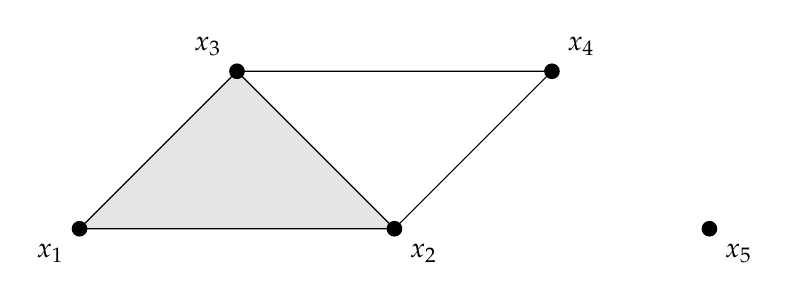
\begin{tikzpicture}

\draw[fill=gray!20] (0,0) -- (2,2) -- (4,0)-- (0,0);
\draw (2,2) -- (6,2) -- (4,0);

\node[circle, fill=black, inner sep=2pt, label=below left:$x_1 $] (a) at (0,0) {};
\node[circle, fill=black, inner sep=2pt, label=above left:$x_3 $] (b) at (2,2) {};
\node[circle, fill=black, inner sep=2pt, label=below right:$x_2 $] (c) at (4,0) {};
\node[circle, fill=black, inner sep=2pt, label=above right:$x_4 $] (c) at (6,2) {};
\node[circle, fill=black, inner sep=2pt, label=below right:$x_5 $] (c) at (8,0) {};




\end{tikzpicture} \end{center}

\end{example} 

\subsection{Simplicial Homology}

~~~Let $\Delta$ be a simplicial complex on $\{x_{1},\dots,x_{n}\}$.
For $i\in\mathbb{Z}$, let 
\[
S_{i}(\Delta):=\text{Span}_{K}\left(\sigma\in\Delta\mid\text{dim}(\sigma)=i\right)\quad\text{and}\quad S(\Delta):=\bigoplus_{i\in\mathbb{Z}}S_{i}(\Delta).
\]

Then $S(\Delta)$ is a graded $K$-module. Let $\partial:S(\Delta)\to S(\Delta)$
be the unique graded endomorphism of degree $-1$ such that 
\[
\partial(\sigma)=\sum_{\lambda\in\sigma}\sigma\backslash\{\lambda\}.
\]
By a direct calculation, we have $\partial^{2}=0$, and so $(S(\Delta),\partial)$
forms a chain complex over $K$; it is called the (\textbf{augmented
}or \textbf{reduced}) \textbf{chain complex of} $\Delta$ \textbf{over
$K$}. The $i$th homology of $(S(\Delta),\partial)$ is called the
$i$\textbf{th reduced homology }of $\Delta$ over $K$, and is commonly
denoted as $\widetilde{H}_{i}(\Delta,K)$.

\begin{example}\label{example} For $\Delta$ as in Example~(\ref{examplesimplicialcomplex}),
we have 
\begin{align*}
S_{2}(\Delta) & =\{\{1,2,3\}\}\\
S_{1}(\Delta) & =\{\{1,2\},\{1,3\},\{2,3\},\{2,4\},\{3,4\}\}\\
S_{0}(\Delta) & =\{\{1\},\{2\},\{3\},\{4\},\{5\}\}\\
S_{-1}(\Delta) & =\{\emptyset\}
\end{align*}

Choosing bases for the $S_{i}(\Delta)$ as suggested by the ordering
of the faces listed above, the chain complex for $\Delta$ becomes
\begin{center}\begin{tikzcd}[ampersand replacement=\&] 

0 \arrow[r] \& K \arrow[swap]{rr}{\begin{pmatrix} 1 \\ 1 \\ 1 \\ 0 \\ 0 \end{pmatrix} } \& \& K^5 \arrow[swap]{rrrr}{ \begin{pmatrix} 1 & 1 & 0 & 0 & 0 \\ 1 & 0 & 1 & 1 & 0 \\ 0 & 1 & 1 & 0 & 1  \\ 0 & 0 & 0 & 1 & 1 \\ 0 & 0 & 0 & 0 & 0 \end{pmatrix} } \& \& \& \& K^5 \arrow[swap]{rrr}{\begin{pmatrix} 1 & 1 & 1 & 1 & 1 \end{pmatrix} } \& \& \& K \arrow[r] \& 0



\end{tikzcd}\end{center}

For example, $\partial_{2}(e_{\{1,2,3\}})=e_{\{2,3\}}+e_{\{1,3\}}+e_{\{1,2\}}$,
which we identify with the vector $(1,1,1,0,0)$. The mapping $\partial_{1}$
has rank $3$, so $\widetilde{H}_{0}(\Delta;K)\cong\widetilde{H}_{1}(\Delta;K)\cong K$
and the other homology groups are $0$. Geometrically, $\widetilde{H}_{0}(\Delta;K)$
is nontrivial since $\Delta$ is disconnected and $\widetilde{H}_{1}(\Delta;K)$
is nontrivial since $\Delta$ contains a triangle which is not the
boundary of an element of $\Delta$. \end{example} 
\end{document}
